% !TEX encoding = MacOSRoman
%\documentclass[10 pt, compsoc]{ieeeconf}
%\newcommand{\CLASSINPUTbaselinestretch}{0.96}
%\documentclass[conference, compsoc]{IEEEtran}
\documentclass[10pt, conference, compsocconf]{IEEEtran}
%\documentclass[10 pt, compsoc]{ieeeconf}
\usepackage{setspace}
%\usepackage{natbib}
%\usepackage[sort]{cite}
\usepackage{graphicx}
\usepackage{times}
\usepackage{subfig}
%\usepackage[noend]{algorithmic}
%\usepackage{algorithm}
\usepackage{url}
\newcommand{\tableref}[1]{Table~\ref{tab:#1}}
\newcommand{\figref}[1]{Figure~\ref{fig:#1}}
%\usepackage[lmargin=1.65cm,rmargin=1.65cm,tmargin=1.8cm,bmargin=2.0cm]{geometry}
\usepackage{amsthm}
\usepackage{amsmath}

\newtheorem{definition}{Definition}
\newtheorem{proposition}{Proposition}
\newtheorem{theorem}{Theorem}
\newtheorem{corollary}{Corollary}
\newtheorem{remark}{Remark}
\newtheorem{lemma}{Lemma}
%\linespread{0.95}

%\renewcommand{\floatpagefraction }{0.9}

\begin{document}

\title{Inferring High-Level Human Behavior 
from Low-Cost Binary Sensors 
}

\author{

\IEEEauthorblockN{
Yuze Lang, Ruoyu Li\\
\IEEEauthorblockA{Department of Electrical and Computer Engineering, Carnegie Mellon University\\ }}
%\{akandhal, raj\}@ece.cmu.edu\vspace{-20pt}}\\
}

\maketitle

\begin{abstract}
Automatic interpretation and prediction of human behavior using pervasive sensors deployed in the environment has a wide variety of applications ranging from building energy minimization, assisted living systems for elders to surveillance. A lot of focus has been given to using information rich sensors such as cameras for these purposes. However, they are expensive, requires careful planning of deployment, and do not preserve the privacy of the user. For these reasons, we propose the use of low cost binary sensors i.e. simple ``on/off" sensors such as motion detectors, status-reporting light switches and so on. Such a system apart from being inexpensive, can be installed easily by end user and is also less invasive. We then show the feasibility of using such sensors for human behavior detection by deploying them in a home, designing an algorithm for modeling the sampled data and then determining human occupancy as well as specific activities. 
\end{abstract}


\section{Introduction}

Detecting human behavior has been of interest in the research community for long now. Knowledge of human behavior can be used in a wide variety of applications, ranging from building automation to surveillance. 
Extensive focus has been placed on using cameras for this purpose. For example, computer vision techniques for behavior detection that uses one or many camera sensors have been proposed in \cite{1}. The authors propose the use of spatio-temporal volumes of force flow to model behavior of crowds. Using this method, they go on to detect and localize abnormal behaviors in crowd videos. \cite{2} provides a survey of vision techniques for human behavior analysis using cameras sensors and computer vision techniques. However, information rich sensors such as cameras and microphones can be expensive. Also they require careful planning during the deployment stage, for example in the case of cameras occlusion can cause the cameras field of view to be blocked due to certain objects and so on. Another major drawback is the fact that they do not maintain the anonymity of the human beings raising huge privacy concerns. Such privacy concerns results in the system not being used at all to begin with.

In order to overcome these drawback, we propose the use of low cost binary sensors i.e. ``on/off" sensors such as motion detector, light switches and so on. These kind of sensors are inexpensive and can be easily installed by end users with minimal amount of configuration. Also, they may seem less invasive and protect the privacy of the end users. We believe that systems using such sensors will be adopted more quickly. However, binary sensors only provide two states of information. Hence, it is not clear if it is enough to determine high level human behavior such as abnormal activity and occupancy that can be detected using cameras. In order to demonstrate the feasibility of using binary sensors, we deploy a set of wirelessly connected binary sensors in a home as shown in Figure \ref{fig:floor}. We collect the sampled data from different types of binary sensors over 7 days. We then model the wireless binary sensor network as a Markov system and use Hidden Markov Model (HMM) to automatically detect the occupancy of the rooms within the home, abnormal human activities and appliance usage information.
 
\section{Related Work}
Monitoring and classification of human activity has been tried to be performed using computer vision techniques via information gathered from camera sensors. \cite{2} provides summary of those techniques. Using other sensors such as microphones, device energy meters, motion detectors has also been studied. In \cite{rowe}, appliance state detectors and plug-load energy meters are used to track the usage pattern of home appliances. 
In \cite{4}, the authors propose the use of many motion sensors to model human activity. Then the transition probability of the sensor states and transition duration time distribution is used as a the template of daily human activity. However, using only motion sensors can be ineffective as they can produce many false-(negatives or positives) due to occlusion or motion of other objects within their field-of-view.
Combining multiple sensors would be much more effective in reducing inaccurate classifications.
Observe that most of these methods exhibit the problems we have discussed in Section 1 i.e. expensive, deployment difficulty, privacy concerns or lack of sufficient accuracy. 

 
\section{System Deployment and Architecture}
In this section, we will describe our wireless binary sensor network deployment in a home and the architecture of the system used to collect the sampling data.
The floor plan of the deployment scene is shown in Figure \ref{fig:floor}. The system architecture is shown in Figure \ref{fig:arch}. 

We place the server in one corner of dinning room to keep it in the geometrical center of the sensor network. Three force sensing resistors are placed under the couch to detect if there is anyone sitting on the couch. Two motion sensors are placed at two enties of the dining room monitoring people walking in and out the dining room. A photo sensing resistor is placed in dining room also to detect if the light of dining room is on. We set the threshold correctly so that the sun light coming in during day time will not confuse the sensor. A motion sensor and a photo sensing resistor are placed in bedroom to detect human activity in the bedding room and the light. A limit switch is attached to the door of the bed room, so that the openness of the door is detected. Two other motion sensors are place in the gate area and hall way to detect if people pass by.

In our paticular scenario, people sitting on the couch only when they are either watching movies or palying Play Station 3, which are both using the projector in the living room. Thus, we did not place a sensor to detect the status of the projector.We planned on installing sensors in bathroom, but since we figured out that would be too personal and privacy related, we did not monitor the status of the bathroom. We planned on to construct an Ad hoc network but then we figured out it is unnecessary since the ability of ZigBee network penetrating wall is quite high and the server is able to receive data from every single sensor.

To collect the data, we designed a data-pull model. Each sensor has a unique id. Since the ZigBee network is broadcasting, the server would send out a comment of pulling data with an argument of sensor id. The sensor receiving that command with the corresponding id would send back the binary status along with its id. Server would log this data into a log file in file system with a time stamp. The time interval of pulling data out is 4 seconds.

Force sensing resistors, photo sensing resistors and limit switches are sending the real time status when they recieve pulling comments. We designed this since sitting on the couch, keeping the light on, or keeping the door closed would not disappear or changed in a short period of time. The delay of acknowledgement when the status changed, which would be no more than 40 seconds, is acceptable in our case. However, the motion sensor would store the status when people pass by until it send the status out. This avoids that when a motion detected, the data is not pulled by the server and the motion is lost and not logged.
\begin{figure}
\begin{center}
%\vspace{-20pt}
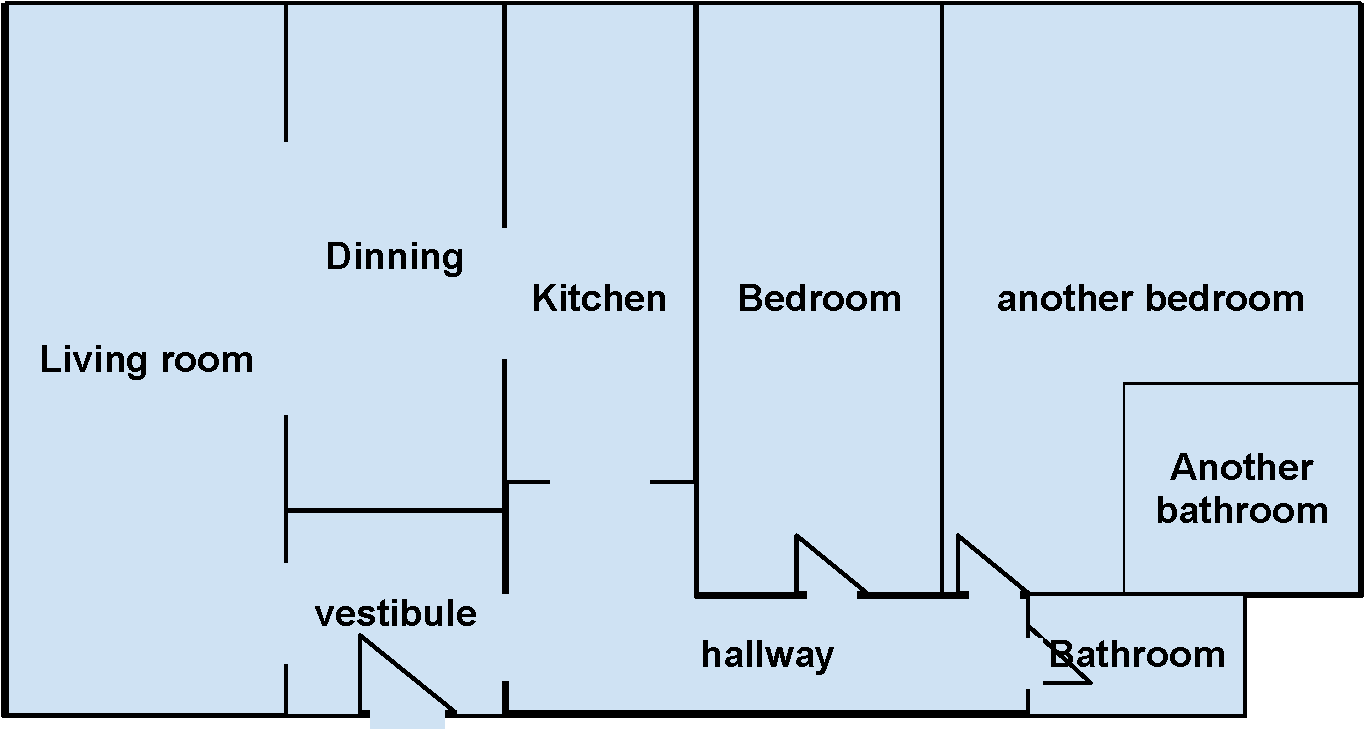
\includegraphics[width=0.7\columnwidth]{figs/floor1-crop}
\end{center}
%\vspace{-14pt}
\caption{Floor plan of home used for our deployment.}
\label{fig:floor}
%\vspace{-4pt}
\end{figure}

\begin{figure}
\begin{center}
%\vspace{-20pt}
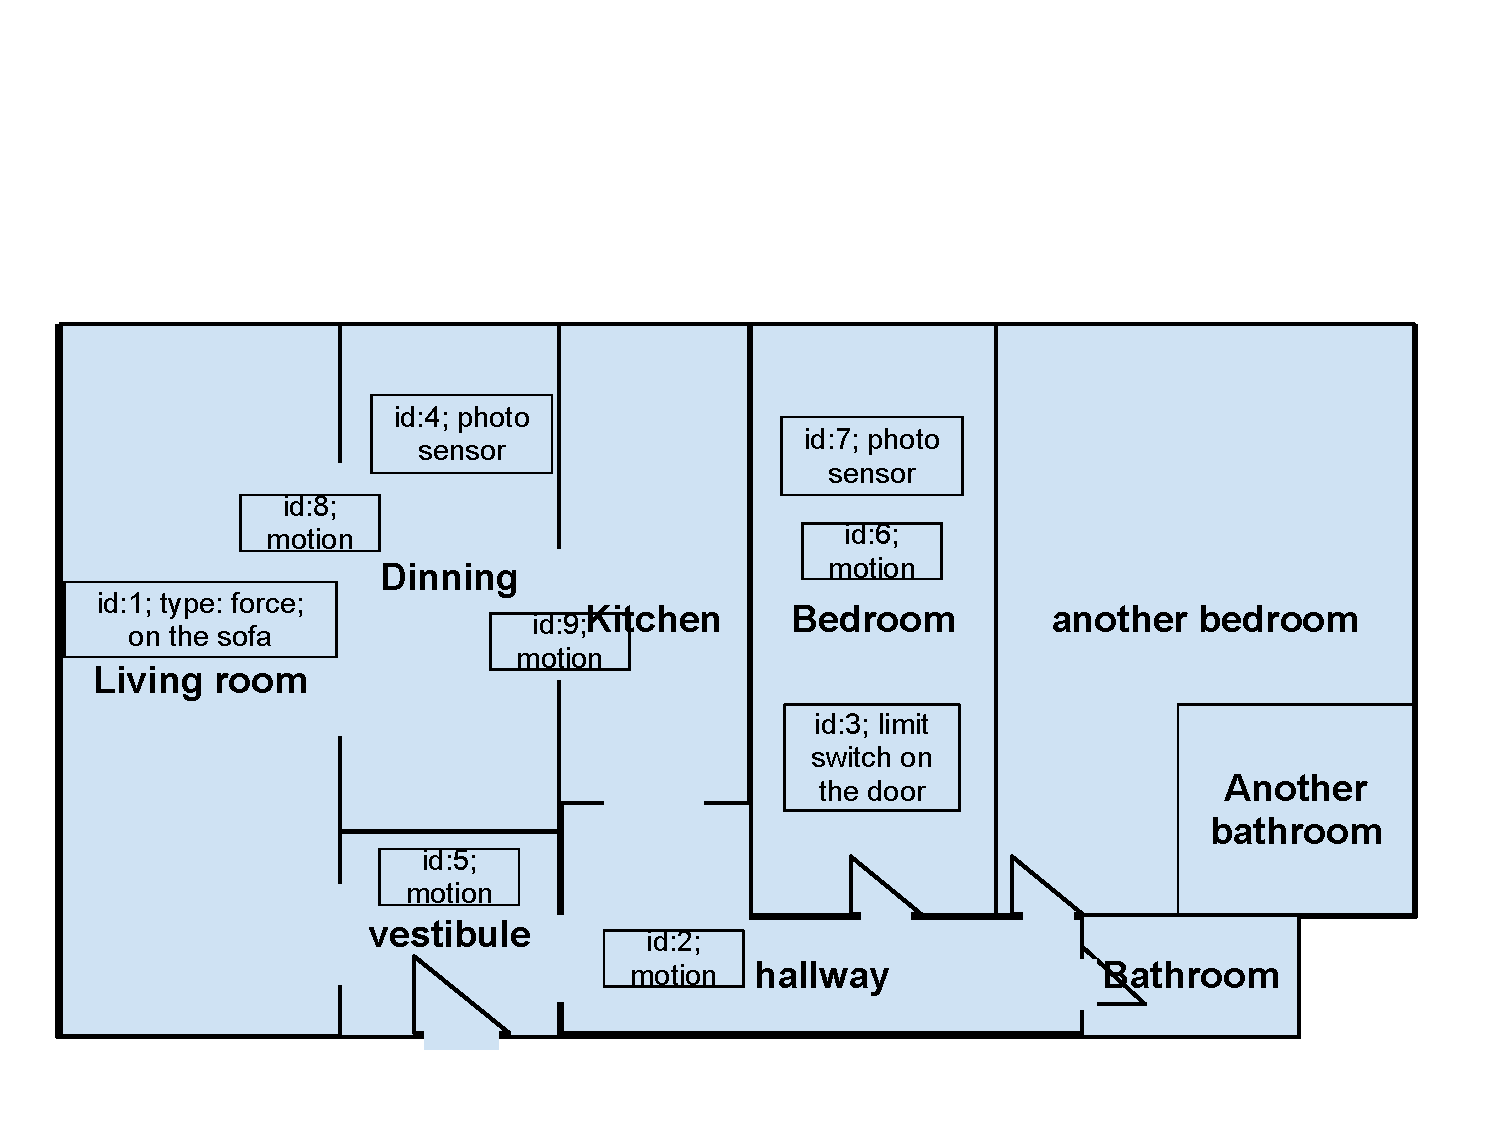
\includegraphics[width=0.8\columnwidth]{figs/sensor-plan}
\end{center}
%\vspace{-14pt}
\caption{Sensor deployement plan.}
\label{fig:floor}
%\vspace{-4pt}
\end{figure}

\begin{figure}
\begin{center}
%\vspace{-20pt}
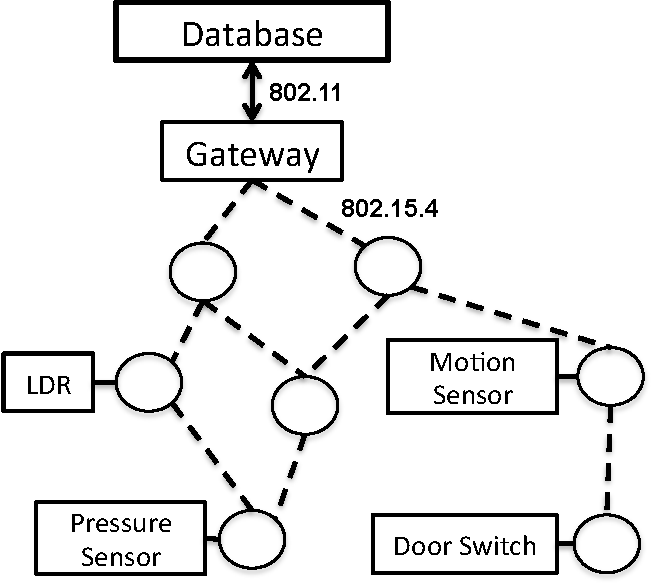
\includegraphics[width=0.5\columnwidth]{figs/arch-crop}
\end{center}
%\vspace{-14pt}
\caption{Architecture of the deployed system.}
\label{fig:arch}
%\vspace{-14pt}
\end{figure}
%\vspace{-6pt}

We use the following sensors: (1) motion sensors (2) light dependent resistors (LDR) (3) pressure sensors (4) door switch. Each of these sensors are coupled with a micro controller and a IEEE 802.15.4 radio (Arduino and Xbee) which form a multi-hop network. In our deployment we needed only a maximum of two hops for covering the entire house. The sampled data from the sensors is transmitted across the 802.15.4 network to a central gateway which is then connected to a database server over a IEEE 802.11 network link. Additionally, each of the sampled data is time-stamped at the gateway before being entered into the database. Our behavior interpretation algorithm will ideally be running on the machine that the database is hosted. In this manner data is collected over seven days.  

\section{Sensor Network Modeling and Human Activity Prediction}
We use a number of sensors deployed across the house. Note that there can be more than one sensor of the same type covering the same area. For example, there can be more than one motion sensor with the same room. We simultaneously need to determine current location of the occupant within the house as well as his/her activity i.e. the occupant {\it state} needs to be updated given sensor measurements. Bayes' filter has been used in the past to estimate the state of a dynamic system from noisy sensor data in real world domains \cite{bayes}. The {\it state} represents occupant location and activity, while sensors provide information about the state. A probability distribution, called the {\it belief}. describes the probability that the occupant is in each state $p(X_t = x_t)$. A Bayes filter updates the belief at each time step, conditioned on the data. Modeling systems over time is made tractable by the Markov assumption that the current state depends only on the previous state.

We estimate the state $x_t$ of an occupants at time using the sensor measurements collected so far, $z_{1:t}$. At each time step we receive the status of many binary sensors. The measurement $z_t = \{e_{1t}, e_{2t}, ..., e_{Et}\}$ is a string of $E$ binary digits representing which sensors have triggered during time step $t$. Rooms provide a natural and intuitive discretization of possible occupant locations. The update equation is analogous to the forward portion of the forward-backward algorithm used in Hidden Markov Models (HMMs). Please see \cite{hmm} for detailed description of how HMMs work. Having multiple occupants complicates the problem further requiring data association to each occupant. In this work, we assume that there is only one occupant. 

We use two separate models, one for sensors called the {\it sensor model} that provide information on the stationary activity of the occupant and the other called the {\it motion model} that tracks the location of the person.
In essence the sensor model $p(z_t|X_t = x_t)$ represents the likelihood of measurement $z_t$ occurring from state $x_t$. 
The motion model $p(X_t = x_t|X_{t-1} = x')$ predicts the likelihood of transition from the state $x'$ to the current state $x_t$. The motion model can further be represented as $p(a_t,r_t|a_{t-1}, r_{t-1})$ = $p(a_t|a_{t-1}, r_{t-1})p(r_t|r_{t-1}, a_{t-1})$, where:
\begin{itemize}
\item{$p(a_t|a_{t-1}, r_{t-1})$ models the probability of whether or not the occupant is moving given the previous room and whether the occupant was moving during the last time step.}
\item{$p(r_t|r_{t-1}, a_{t-1})$ is the probability of transition to a room given the previous room and whether the occupant was moving or not.}
\end{itemize}
Note that here, the state space $x \in X$ for an occupant is the range of possible locations and activities, $x_t = {r_t, a_t}$, where $r \in R$ denotes which room the occupant is in, and $a \in \{$moving, not moving$\}$ denotes occupant activity. Although, $a$ is shown here to comprise only movement activity it of course can incorporate many other types of activities depending on the sensors. In our system, we consider sitting, watching TV, Sleeping, Switching ON/OFF lights apart from movement activity. The raw sensor values are the only given information and the rest must be inferred. The graphical representation of our model is shown in Figure \ref{fig:graph}.

\begin{figure}
\begin{center}
%\vspace{-20pt}
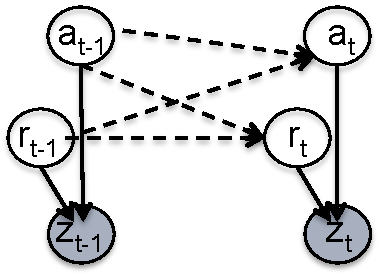
\includegraphics[width=0.35\columnwidth]{graph-crop}
\end{center}
%\vspace{-14pt}
\caption{Markov representation of our system. The lines represent the causal influences, while the dotted-lines represent the causality through time. The circles represent the variables. Shaded variables are directly observable i.e. the measured data, the rest are hidden.}
\label{fig:graph}
%\vspace{-14pt}
\end{figure}

Apart from the sensor data, the time stamp information can further be used to classify as well as detect abnormal events. The time at which a state occurs as well as the duration of the state can be used to classify activity. For example, movement across at 4 A.M or sleep state for longer than usual durations can be detected as abnormal activities. Also space i.e. location can also be used for detecting abnormalities. While detecting sleep state in bedroom is okay, detecting sleep state for example in bathroom can be an abnormality. In this manner, time as well as space information can be used for further classification and abnormality detection.
%For this, we first need to ``fuse" the information from orthogonal binary sensors such as motion sensors and light sensors across time as well as space to {\it detect} an event. Then, once the sensor data is fused then an interpretation algorithm will determine the {\it type} of event.
%\subsection{Sensor Fusion}
%The sensor fusion is used to detect an event. For example, motion sensors along with light sensors and door sensors can determine if a person walked in to a room and so on. The fusion of multiple sensors is required to reduce the false positives arising in event detection using binary sensors if only one type of sensor is used. 
%In order to perform fusion, we use correlation filters. We expect sensors that are placed within close proximity of each other to exhibit strong correlation (positive or negative) in time when an event occurs.
%
%\subsection{Interpretation}
%After an event is detected then the type of event needs to be detected. For this purpose, both the time as well as location information is used. For example, the presence of a person in bed room can be detected using motion sensors and information whether the lights are switched on or not can be obtained using the light sensors. Then, combining it with the time-stamp information of the sampled data, one can predict if the person is sleeping or not. Such an event classification is probabilistic in nature. Bayes' filters offer a well known way to estimate the state of a dynamic system from noisy sensor data in real work domains. 
%


\section{Evaluation}
We evaluate the performance of our system in this section. 

Figure \ref{fig:data} shows the sampled data over a short span of time (7.26.16 PM to 7.26.52 PM) on a particular day with a sampling frequency of 4 seconds. The data is collected from the motion, light and pressure sensor deployed in the bedroom. Light sensor is used to determine if the lighting in the room is switched ON, and the pressure sensor is essentially a limit switch that determines if the room door is shut or not. 
From figure \ref{fig:data} the following sequence may be inferred. There is motion in the room at 7.26.16 indicating the presence of a person. The door is shut and then the light is switched on. This could mean that either the person will be studying in the room or will be going to sleep and so on. In this manner we observe that using simply binary sensors deployed across the apartment, the occurrence of an event as well as the type of event could possibly be determined. As mentioned in the previous section, we use HMMs to perform the event estimation from the collected data.

We have collected data over 7 days and used to for training our proposed HMM (given in previous section) as well as for evaluating the estimation accuracy.
The accuracy of the event estimation obtained using our HMM trained from our collected data is shown in Figure \ref{fig:plot1-crop}. 
The couch corresponds to a person sitting on the couch in living room and ``$>$ 1" indicates the detection of presence of more than one person in the apartment.
We observe that using the time of event and duration of an event helps in improving the estimation accuracy for certain types of events. For example, the time and duration of the ``sleep event" helps in improving the detection accuracy from ~60\% to ~90\%. 

Figure \ref{fig:plot2-crop} shows the detection accuracy with using motion sensor alone and using fused information from multiple sensors.
Note that the all the results for this figure are obtained without using time information. In the case of sleeping event, light sensors as well as pressure sensors on the door are used for the fused case. In the case of studying event, motion and light are used. For dining event we see that motion sensor alone gives good accuracy and using a light sensor only improves it by a small margin. This could be attributed to the fact that the dining room is used only for that purpose and the light as well as motion sensors are invariably triggered only for this event.

\begin{figure}
\begin{center}
%\vspace{-20pt}
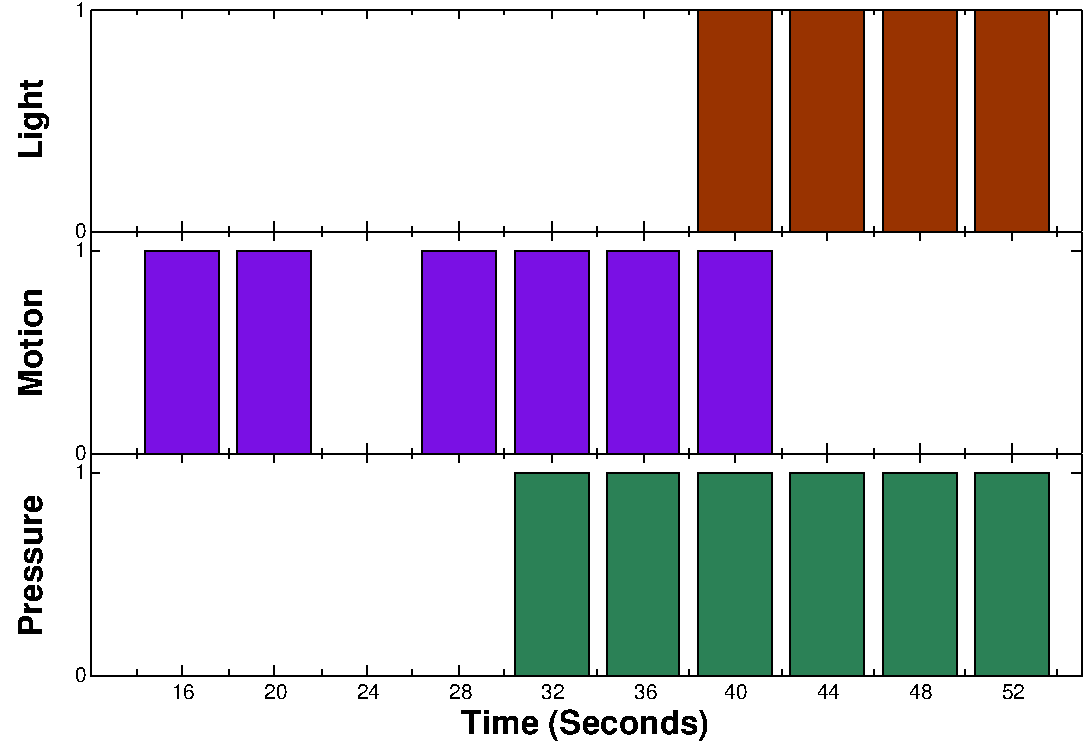
\includegraphics[width=0.7\columnwidth]{event-tv-crop}
\end{center}
%\vspace{-14pt}
\caption{Sampled data over 7.26.16 PM to 7.26.52 PM on a day for three different sensors in a room. Sampling frequency is 4 seconds.}
\label{fig:data}
\vspace{-4pt}
\end{figure}

\begin{figure}
\begin{center}
%\vspace{-20pt}
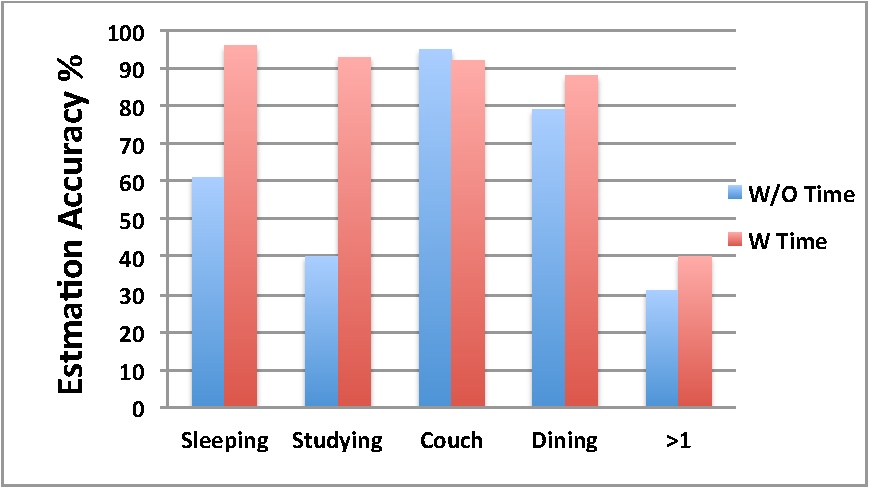
\includegraphics[width=0.7\columnwidth]{plot1-crop}
\end{center}
%\vspace{-14pt}
\caption{Detection accuracy for different types of events from HMM with and without (w/o) time information.}
\label{fig:plot1-crop}
\end{figure}

\begin{figure}
\begin{center}
%\vspace{-20pt}
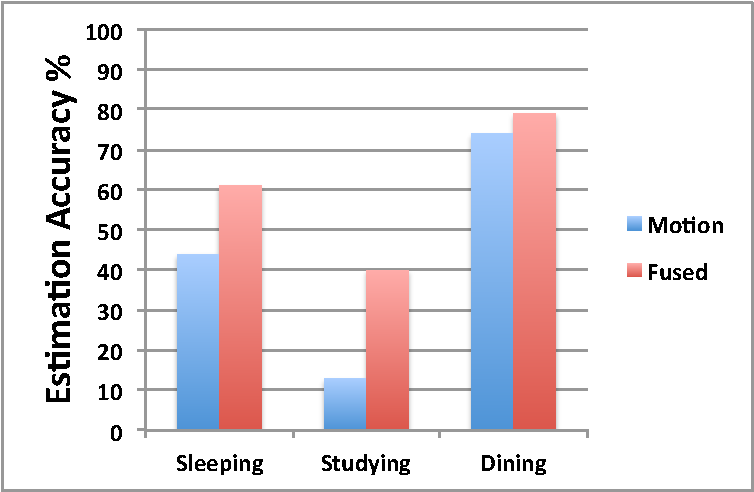
\includegraphics[width=0.7\columnwidth]{plot2-crop}
\end{center}
%\vspace{-14pt}
\caption{Detection accuracy from HMM using only motion sensor and using motion sensor fused with other sensors such as light and pressure sensors.}
\label{fig:plot2-crop}
\end{figure}


\section{Conclusion and Future Work}
In this work, we have proposed the use of binary sensors for detecting and classifying events related to human behaviors. This has a wide variety of applications and using binary sensors has the following advantages: inexpensive, ease of deployment and privacy protection. We have deployed out system and show that behavior detection can be feasibly performed using our HMM based algorithm. In this work, we assumed that there is only one occupant and also the deployment duration was only for a week. As future work, we will collect data over longer durations and consider multiple occupant scenarios.
Additionally there has been work on using network activity for determining building occupant models. For example, in \cite{wifi} the authors propose monitoring the IP traffic of existing network infrastructure to determine the building occupancy. Then the occupancy information can be used to minimize the building energy consumption by controlling the lighting and HVAC systems automatically. We believe that integrating binary sensors with existing network monitoring can be effective in determining human behavior.

\section{Acknowledgements}
We would like to thank Yuze Lang and his two suitemates for letting us use their apartment for our experiments. We also thank Pei and Rajeev for their guidance and useful insights.

 
%\vspace{-5pt}

%\setlength{\bibsep}{0pt}
%\bibliographystyle{IEEEtran}
\begin{thebibliography}{9}
\bibitem{1}{Ramin Mehran et. al, ``Abnormal Crowd Behavior Detection using Social Force Model", {\it CVPR} 2009.}
\bibitem{2}{Julio et. al., ``Crowd Analysis Using Computer Vision Techniques", {\it IEEE Signal Processing Magazine} 2010.}
\bibitem{hmm}{L. Rabinder, ``A tutorial on hidden markov models", {\it Proceedings of IEEE} 1989.}
\bibitem{4}{Hara, K, ``Detection of unusual human behavior in intelligent house", {\it Neural Networks for Signal Processing} 2002.}
\bibitem{5}{Mickael et. al., ``Indoor Location Tracking based on a Discrete
Event Model", {\it International Conference on Smart Homes and Health Telematics} 2012.}
\bibitem{6}{Elliot Cohen and John Canny, ``Modeling human behavior from simple sensors in the home", {\it Pervasive Computing} 2006.}
\bibitem{wifi}{Ryan Melfi, Ben Rosenblum, Bruce Nordman, and Ken Christensen, ``Measuring Building Occupancy using Existing Network Infrastructure", {\it Green Computing} 2011.}
\bibitem{rowe}{Mario Berges, Anthony Rowe, ``Appliance Classification and Energy Management Using Multi-Modal Sensing,"  {\it BuildSys}, 2011.}
\bibitem{bayes}{A. Doucet, N. de Freitas, and N. Gordon, {\it ``Sequential Monte Carlo in Practice"}, 2001.}
\end{thebibliography}

%
\end{document}
